\section{Deskriptor}
Fra en detektor genereres et sæt interessepunkter $p$ fra to eller flere billeder $I$:
$$ Det(I) = \lbrace p_1,p_2,...,p_n \rbrace $$
\vspace{-1em}
$$
Det(I') = \lbrace p_1',p_2',...,p_n' \rbrace
$$
For at udvælge korresponderende punkter imellem billederne, skal interessepunkterne beskrives af en deskriptor "$Des$". Deskriptoren tager et billede og et punkt, og beskriver dette punkt, udefra noget lokalt billeddata<klare?>, omkring punktet. Den tilegnede beskrivelse kaldes en "Feature" $F$:
$$ Des(I,p_i)=F_i $$
For to korresponderende punkter $i$ og $j$ ønskes det at $F_i \approx F'_j$, så punkterne korrekt kan identificeres som korrespondancer, men også for to \textit{ikke} korresponderende punkter $k$ og $l$ at $F_k \not\approx F'_l$ så de kan identificeres som ikke korresponderende. Den tilegnede beskrivelse kommer ofte i form af en n-dimensional vektor\footnote{For en given metode vil længden af disse vektorer være ens}, hvor indgangende i vektoren indeholder information om området omkring interessepunktet, hvilket kan bruges til at determinere, ligheden af interessepunkterne.
$$ F =
\begin{bmatrix}
d_1 \\
d_2 \\
. . . \\
d_n
\end{bmatrix}
$$
En simpel metode at beskrive et interessepunkt på, er at udvælge et $n \times n$ område omkring punktet og gemme disse pixel værdier i en vektor. Dette kan være fordelagtigt, hvis de to billeder ikke er udsat for ændringer, andet end forkydelse af kameraet. Men da billederne næsten i alle sammenhæng med fotografering, undtagen i meget kontrollerede forhold, udsættets for mange forskellige ændringer, når kameraet skifter position, vil denne løsning ikke virke. Generelt ønskes der at en deskriptor besidder følgende egenskaber:
\begin{itemize}
\item{\textit{Robust}: Deskriptoren skal kunne identificere to korresponderende punkter som værende ens på trods af transformationer i billedet, som ændringer i lys}
\item{\textit{Invariant}: Deskriptoren skal være invariant overfor geometriske transformationer som skalaændringer og rotation.}
\end{itemize}
Roationsinvarians kan opnås ved at finde den dominerende gradient i pixelområdet, omkring interessepunktet og derved punktets orientering. Regionen kan dernæst roteres ift. punktets orientering \cite{bjerg}. Dette er illustreret i figur \ref{fig:bjerg}, hvor regionen omkring et interessepunkt er roteret relativt til interessepunktets orientering.
\begin{figure}[H]
    \centering
    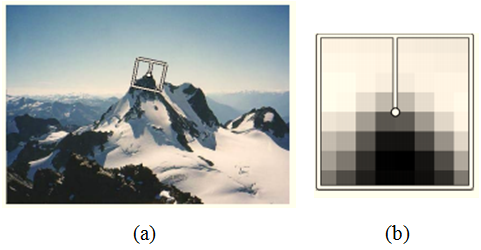
\includegraphics[width=0.45\textwidth]{fig/21.png}
    \vspace{-0.5em} 
    \begin{center}
    \caption{\textcolor{gray}{\footnotesize \textit{
   (a) Et interessepunkt lokaliseret på en bjergtop,  repræsenteret af en firkant, med centrum i interessepunktet og en lodret streg der angiver punktets rotation. (b) Interessepunktet forstørret i et 8x8 pixel område, hvor rotationen af punktet er trukket fra og derfor normaliseret.}}}
    \label{fig:bjerg}
     \end{center}
  \end{figure}
       \vspace{-2.5em}
\noindent
Selv efter kompensering for rotation, skala o.s.v. vil korresponderende regioner stadig variere ift. til hinanden. Udfordringen består derved i at deskriptoren skal være invariant overfor ændringer så korresponderende punkter kan matches korrekt, men også informationsbærende nok, til at undgå forkerte korrespondancer.